\chapter{INTRODUÇÃO}
\label{cap1}

Este relatório tem como objetivo geral apresentar as etapas de modelagem e processamento sísmico de um dado sísmico sintético
utilizando os softwares Seismic Unix (SU) e Matlab.

Apresentaremos um fluxograma (figura \ref{fig:fluxograma}) do processamento de dados sísmicos sintéticos, com a aplicação do método de imageamento sísmico CDP, através do software livre Seismic Unix.

O Seismic Unix é um software de processamento de dados sísmicos de código aberto desenvolvido pelo \textit{Wave Field Research Center}
(CWP) da Escola de Minas do Colorado, usado principalmente para ensino e pesquisa em exploração sísmica.

Desta forma deseja-se obter uma melhor imagem da subsuperfície através das técnicas empregadas ao decorrer deste trabalho. A seguir, apresenta-se um fluxograma típico de processamento de um dado sísmico. Algumas etapas do processamento são opcionais, e a sequência pode ser modificada para se adequar ao trabalho desejado.


\begin{figure}[H]
\centering
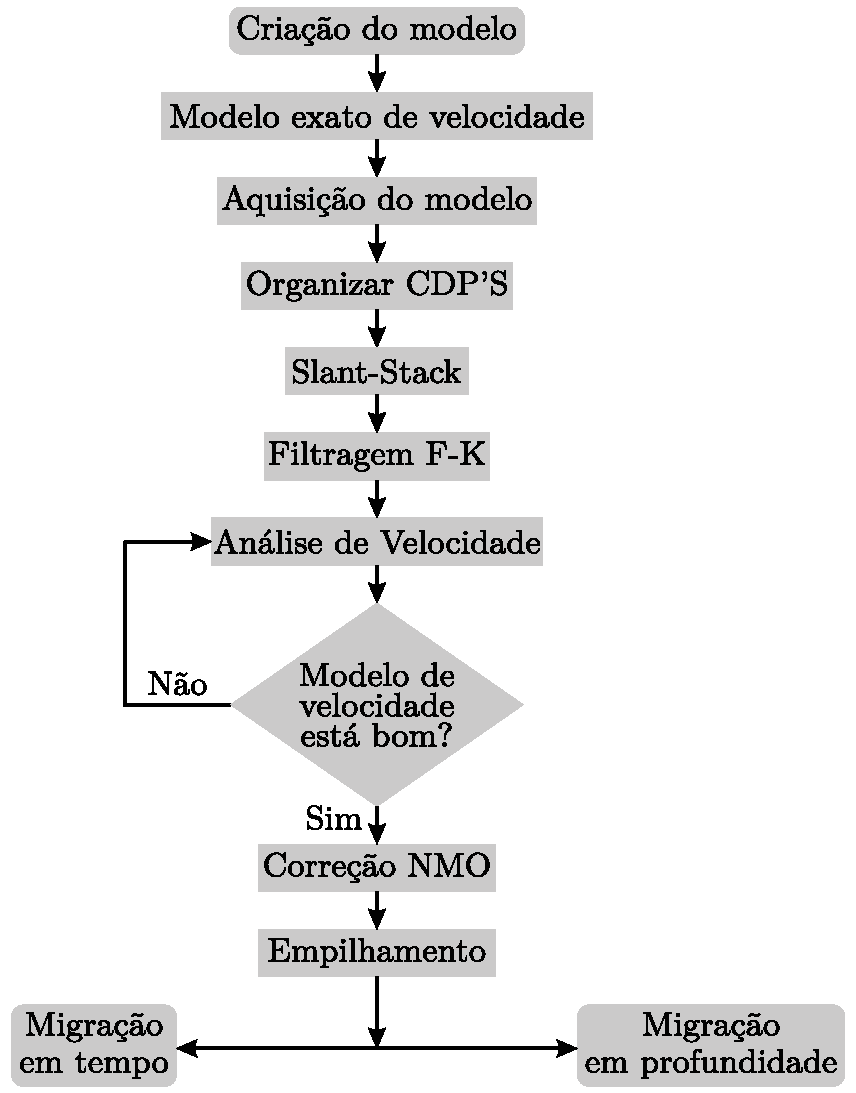
\includegraphics[width=10cm]{figuras/cap1/fluxograma.pdf}
\caption{Fluxograma do processamento adotado neste trabalho.}
\label{fig:fluxograma}
\end{figure}
